\documentclass[journal]{IEEEtran}

\usepackage[T1]{fontenc}
\usepackage{amsmath,amsfonts}
\usepackage{newtxtext}
\usepackage{newtxmath}

\usepackage{algorithmic}

\usepackage{cite}
\usepackage{graphicx}
\usepackage{booktabs}
\usepackage{tabularx}
\usepackage{geometry}

\usepackage{tikz}
\usetikzlibrary{shapes.geometric, arrows, arrows.meta, positioning, calc}

\usepackage[hidelinks]{hyperref}

\begin{document}

\title{Measuring the Effects of White Noise and Music on Anxiety Level Using a Commerical EEG}

\author{Andy Babcock \\
    \textit{Steve Sanghi College of Engineering, Northern Arizona University} \\
    Flagstaff, AZ, USA \\
    aab726@nau.edu
}

\maketitle

\begin{abstract}
text
\end{abstract}

\begin{IEEEkeywords}
Anxiety relief, EEG, electroencephalography, white noise, music.
\end{IEEEkeywords}

Anxiety and anxiety disorders are one of the most prevalent mental health conditions, predominately affecting youth and young adults, ages 10-24~\cite{bieRisingGlobalBurden2024}. In the past 35 years, anxiety disorders have increased by 52\% among adolescents and young adults. Daily anxiety affects nearly all parts of life, and is especially disruptive when under a high cognitive load. A 2007 study examined how anxiety impairs efficient cognitive functioning by taking attention away from the task at hand and instead focusing on the source of the anxiety~\cite{eysenckAnxietyCognitivePerformance2007}. However, the overall quality of performance does not neccessarily suffer, depending on compensatory stragegies used, like intentionally mentally working harder than neccesary. One strategy that requires less intentional mental application is playing white noise: a 2025 study examined how the anxiety levels of college students undergoing Cognitive Behavioral Therapy (CBT) were changed by white noise~\cite{liEffectWhiteNoise2025}. This study focuses on the difference in anxiety, depression, and sleep quality when only undergoing CBT, and while also listening to white noise in therapy. CBT represents a different dynamic to test-taking, but shares some qualities, such as therapy being an innate stessor, which can compound with external stressors (i.e.: needing to set boundaries with family). Anxiety levels in test-taking can be be monitored for changes from external factors like white noise or music using an Electroencephalogram (EEG) to measure changes in brain activity which is correlated to anxiety.

\section{Literature Review}
\subsection{White Noise and Cognitive Load}
A 2022 paper examines the effect of white noise on anxiety in operating room staff~\cite{shahrokhiEffectWhiteNoise2022}. Operating rooms share many similarities with test-taking, presenting both inherent stressors (successfully operating on another human) and external stressors (an expectation for the staff to do their jobs well and quickly). Anxiety reduces performance at work, so any simple solution that could potentially decrease anxiety would represent a painless way to improve performance. Previous studies found that music significantly reduces stress, but also reduces the surgeon's auditory processing~\cite[p.~2]{wayEffectNoiseAuditory2013}. A potential middle ground that addresses this issue are less audible, muffled sounds that draw less attention than music would. Thus, the study chose white noise from a suction machine, which is already commonly used in operating rooms.

The paper tests this hypothesis with a single-blind, crossover clinical trial on staff conducting cesarean sections, both with and without white noise from a suction machine. To test for differences in anxiety, the study measured hemodynamic parameters for the physical signs of anxiety, and used the Spielberger State-Trait Anxiety Inventory to measure anxiety level~\cite[pg.~1]{shahrokhiEffectWhiteNoise2022}. However, the study found no significant difference in anxiety whether the suction machine was running or not. The paper theorized that meaningless sounds like white noise are adapted to in the same way as other operating room noises, reducing its impact~\cite[pg.~3]{shahrokhiEffectWhiteNoise2022}. While these findings are inconclusive, there may be nuance lost in the somewhat chaotic setting of an operating room (chaotic in terms of multiple people talking, multiple sound sources, and a tangible source of high anxiety). 

When isolating study participants with fewer uncontrollable variables, white noise was found to either notably increase sensory overload or to act as a sedative on the brain, likely depending on each individual's mental state and white noise intensity. In the former scenario, participants were tasked with folding a piece of paper into various configurations and difficulties, while introducing up to eight different conditions to mentally exhaust the participant~\cite{marzollaImpactNoiseExposure2024}. The study found that sensory overload generally increased as more conditions were introduced, with white noise having the most signficant impact. However, the assesed level of sensory overload did not effect the participant's performance on the tasks, only their mental state. Alternatively, white noise can have a sedative effect on the prefrontal cortex, which presents as a calming effect~\cite{zhangSedativeEffectWhite2025}. This study differs from the previous two in that the participants were tested in calm, consistent environments, with no test or goal during the experiment aside from sitting in silence or listening to white noise. This format allowed for specific analysis of how white noise causes mental changes, but these positive effects may not be seen under high cognitive loads and anxiety levels.

\subsection{Methods of Measuring Anxiety with an EEG}

Commerical EEGs have high potential for lowering the bar of entry for those interested in studying brainwaves, at the cost of less accurate results. SingLEM is a pre-trained deep learning model trained on 357,000 hours of single-channel commercial EEG data~\cite{sukhbaatarSingLEMSingleChannelLarge2025}. Pre-training a deep learning model on such an expansive number of participants and hours of data allows it to differentiate between the brain signals and noise from blinking or moving. To validate SingLEM, it was tested as a fixed feature extractor; the model was not fine-tuned, and tested in identifying the correct limb in motor imagry tasks and mental states during cognitive tasks. Compared against its predicessors, SingLEM showed a 5-10\% improvement across all tasks. 

Alternatively, the raw electrical signal collected by an EEG can be converted into brainwaves using a Fourier Transformation. A 2017 study found that low Beta waves (12-17Hz) predict the participants percieved stress 94\% of the time, while high Beta waves (18-30Hz) did not predict stress~\cite{muhammadumarsaeedQuantificationHumanStress2017}. Filtering only for Beta waves and using a Naive Bayes machine allowed for accurate stress prediction with low computational cost.

EEGs with multiple sensors have more potential methods of data analysis. Thanks to the sensors being placed in multiple locations, a model could track the fluctuations in each observed feature to account for the distortion inherent to reading brainwaves through the skull. A 2023 study implemented this using an EEG with 14 channels, and tracked Hjorth parameters to measure the properties of the signal over time, sub-band powers like Alpha and Beta waves, and an Engagement Index, a calculated ratio Alpha, Beta, and Theta waves~\cite{chatterjeeDetectionMentalStress2023}. Tracking the changes in these features across the skull allowed the team to generate normalized distributions, allowing for more accurate data collection.

% possibly add MVCA-net, I don't think I'll have space really

% =======
% Q AND H
% =======

\section{Questions and Hypotheses}

The above examined studies on axiety and EEG anxiety assessment provides a solid base to extrapolate how noise would effect anxiety while test-taking. White noise in the operating room showed no difference in anxiety level, while music decreased both anxiety and auditory processing\cite{shahrokhiEffectWhiteNoise2022, wayEffectNoiseAuditory2013}. In an operating room, auditory processing is critical, but in many other stressful situations, it is much less important. In a more controlled scenario, it may be more likely that the white noise would calm the participant~\cite{zhangSedativeEffectWhite2025}.

While performing controlled tasks, what is the effect of white noise on task anxiety? It is likely that listening to white noise shows a statistically significant reduction in anxiety and no change in performance~\cite{zhangSedativeEffectWhite2025}. Though unexpected, anxiety levels may remain the same or rise while listening to white noise and compared to the task done in silence\cite{shahrokhiEffectWhiteNoise2022, marzollaImpactNoiseExposure2024}. Through collecting data using a commercial EEG, we will test the effect of white noise on anxiety-inducing tasks. Additionally, we will repeat the same tasks while listening to music with and without lyrics, and expect no change in performance but a decrease in anxiety~\cite{kissEffectPreferredBackground2021}.

Using a wearable EEG that measures stress, we will test these claims by repeatedly taking tests under various auditory conditions. EEGs have already proven to be accurate in tracking stress, and allow for continuous monitoring throughout test-taking~\cite{sukhbaatarSingLEMSingleChannelLarge2025}. With an EEG, we can track how anxiety levels shift throughout the test-taking process, allowing for insights like when axiety is at its highest, and how much various kinds of noise dampen that peak. To interpret this data, we will fine-tune SingLEM on our collected data, and perform brainwave band analysis, focusing on the Beta band~\cite{sukhbaatarSingLEMSingleChannelLarge2025, muhammadumarsaeedQuantificationHumanStress2017}.

\section{Device Design}

% =============
% device design
% =============

To realize a wearable anxiety monitor, a NeuroSky MindWave Mobile 2 is being used. This headset was released in 2018, and included first-party software support on Windows, Android, and iOS~\cite{neuroskyNeuroSkyMindWaveMobile2018}. To track data, we will use NeuroSky's eegID Android app, which saves all collected data as a CSV~\cite{isomerprogrammingllcEegID2015}. While there are other alternatives, including connecting the headset directly to a computer using a python script or program, the mobile app is sufficient, with all data analysis happening afterwards. Additionally, because eegID has not recieved updates since late 2015, it will be easier to pair it to an older phone - in this case, a Motorola Moto X4, which was released in 2017.

\begin{figure}[htbp]
    \centering
    \resizebox{\columnwidth}{!}{%
    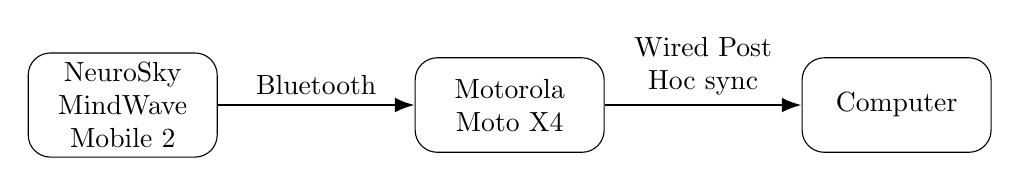
\begin{tikzpicture}[
        node distance=2.5cm,
        auto,
        block/.style={
            rectangle,
            draw,
            rounded corners=8pt,
            minimum width=2.4cm,
            minimum height=1.2cm,
            text centered,
            align=center
        },
        line/.style={draw, -{Latex[length=2.5mm]}, thick}
    ]
        % nodes
        \node [block] (headset) {NeuroSky\\MindWave\\Mobile 2};
        \node [block, right=of headset] (phone) {Motorola\\Moto X4};
        \node [block, right=of phone] (computer) {Computer};

        % paths
        \path [line] (headset) -- node[align=center, above] {Bluetooth} (phone);
        
        \path [line] (phone) -- node[align=center, above] {Wired Post\\Hoc sync} (computer);
        
    \end{tikzpicture}%
    }
    \caption{Hardware data flow and synchronization architecture.}
    \label{fig:data_flow}
\end{figure}

% =============
%  methods plan
% =============

\section{Methods Plan}

To measure anxiety, we will perform two tasks in silence, and while listening to white noise, lyrical music, and lyric-less music. For the purpose of training SingLEM, we will also take data while aware but unstressed. Based loosely off of Peplau's definitions of levels of anxiety, we chose Level 1 to be a cognitively aware baseline, and Level 2 as light anxiety while under cognitive load, with our Level 2 corresponding to Peplau's Level 1~\cite{peplauInterpersonalRelationsNursing1952}. To collect Level 1 data, we chose two tasks: reading a book, and listening to music. For Level 2 data, we chose a modified Stroop test and a Typing test.

The Stroop test traditionally is formatted as a list of words in various colors, sometimes with the words being the names of those colors~\cite{macleodHalfCenturyResearch1991}. The participant must name the color of the word, not the word itself. To avoid the additional movement introduced by speaking, we will instead play the Stroop game using a Python script, with four colors mapped to keys on the keyboard. This game is cognitively challenging by forcing the brain to simultaneously process the word and the color of the word, with the color detection being the much less practiced skill of the two. Additionally, we will implement a correct answer counter, adding inherent pressure as the streak increases~\cite{yamadaExperimentalParadigmManipulate2025}.

Our Typing test is similar to most online typing games, with a feed of words to type as fast as possible. Like the Stroop test, this game will implement a correct word counter to increase anxiety during the test~\cite{yamadaExperimentalParadigmManipulate2025}.

% \begin{table*}[t]
%     \centering
%     \caption{eegID Telemetry Fields and Correlated Brainwave States~\cite{neurosky2026eegid,neurohealth_2019}}
%     \label{tab:eegid_brainwaves}
%     \begin{tabularx}{\textwidth}{l l X}
%         \hline
%         \textbf{eegID Field} & \textbf{Frequency Range} & \textbf{Description and Meaning} \\
%         \hline
%         PoorSignal & N/A & A hardware metric indicating the quality of the sensor contact and signal integrity. \\
%         EEG Raw Value & N/A & Unfiltered analog values captured directly from the EEG sensor. \\
%         EEG Raw Value Volts & N/A & The raw EEG data scaled and converted into standard voltage units. \\
%         Attention Level & N/A & A computed metric (ThinkGear algorithm) measuring the user's focus, concentration, and directed mental effort. \\
%         Meditation Level & N/A & A computed metric (ThinkGear algorithm) measuring the user's level of mental calmness and relaxation. \\
%         Blink Strength & N/A & A metric that detects eye blinks and quantifies their relative physical intensity. \\
%         Delta & 1--3 Hz & Associated with deep, dreamless sleep, trance, and the unconscious mind. Represents a decreased awareness of the physical world. \\
%         Theta & 4--7 Hz & Linked to intuition, creativity, daydreaming, internal focus, and spiritual awareness. Reflects the state between wakefulness and sleep. \\
%         Alpha Low & 8--9 Hz & Correlates to an inner-awareness of self, mind/body integration, and balance. \\
%         Alpha High & 10--12 Hz & Associated with centering, healing, and bridging the conscious to the subconscious. Promotes mental resourcefulness and calmness. \\
%         Beta Low & 13--17 Hz & Reflects a state of being relaxed yet focused, integrated, and actively thinking while remaining aware of surroundings. \\
%         Beta High & 18--30 Hz & Indicates high alertness and mental activity (e.g., math, planning), and general activation of mind/body functions, but can also reflect agitation. \\
%         Gamma Low & 31--40 Hz & Consolidates information from different areas of the brain for simultaneous processing. Associated with alertness, good memory, or potential agitation. \\
%         Gamma Mid & 41--50 Hz & Functions similarly to Gamma Low in consolidating rapid, simultaneous processing across brain regions; also indicates high alertness or agitation. \\
%         \hline
%     \end{tabularx}
% \end{table*}

\subsection{Collecting Data}

We will use a NeuroSky Mindwave Mobile 2 to collect data and follow the included instructions for positioning: the sensor over the left eyebrow and ground clip on the left ear~\cite{neuroskyNeuroSkyMindWaveMobile2018}. When initially putting on the headset, we will readjust it until the 'Poor Signal' field drops to 0, and quickly returns there after blinking. We then set the recording limit to '5 minutes', and the recording interval to 'All'. All data will be collected in the same room, sitting at a desk in front of a computer. When the computer is not being used, it will be off. If the Stroop or Typing test is being taken, we will start the EEG recording first, then start the game on the computer. If white noise or music is needed, it will be played through wireless earbuds.

\subsection{Methods of Measuring Anxiety}

\begin{figure}[!t]
    \centering
    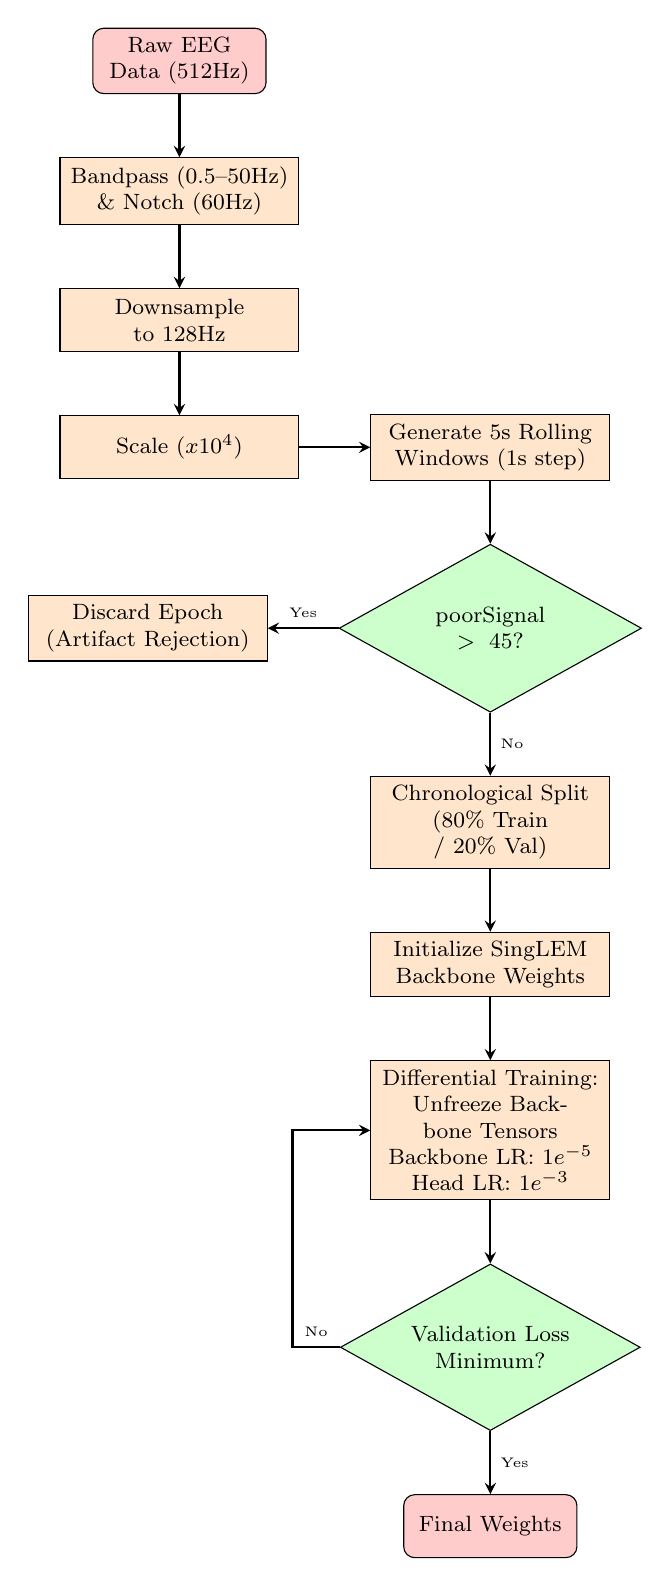
\begin{tikzpicture}[
        node distance=0.8cm and 0.6cm, % Tighter spacing for standard column width
        auto,
        % styles
        startstop/.style={rectangle, rounded corners, minimum width=2.2cm, minimum height=0.8cm, text centered, draw=black, fill=red!20, font=\footnotesize, align=center},
        process/.style={rectangle, minimum width=2.5cm, minimum height=0.8cm, text centered, text width=2.8cm, draw=black, fill=orange!20, font=\footnotesize, align=center},
        % decision/.style={diamond, aspect=1.8, minimum width=2cm, minimum height=0.8cm, text centered, text width=1.8cm, draw=black, fill=green!20, font=\tiny, align=center},
        decision/.style={diamond, aspect=1.8, minimum width=2.5cm, minimum height=0.8cm, text centered, text width=2.2cm, draw=black, fill=green!20, font=\footnotesize, align=center},
        arrow/.style={thick,->,>=stealth} ]

    % --- COLUMN 1: Preprocessing ---
    \node (start) [startstop] {Raw EEG\\Data (512Hz)};
    \node (pro1)  [process, below=of start] {Bandpass (0.5--50Hz)\\ \& Notch (60Hz)};
    \node (pro2)  [process, below=of pro1] {Downsample\\to 128Hz};
    \node (pro3)  [process, below=of pro2] {Scale ($x 10^4$)};

    % --- COLUMN 2: Windowing & Training ---
    % Shift to the right to start the second column
    \node (pro4)  [process, right=of pro3, xshift=0.3cm] {Generate 5s Rolling\\ Windows (1s step)};
    \node (dec1)  [decision, below=of pro4] {poorSignal $> 45$?};
    
    % Back to Column 1 space (tucked under pro3) for the discard node
    \node (pro5)  [process, left=of dec1, xshift=-0.3cm] {Discard Epoch\\(Artifact Rejection)};
    
    \node (pro6)  [process, below=of dec1] {Chronological Split\\(80\% Train / 20\% Val)};
    \node (pro7)  [process, below=of pro6] {Initialize SingLEM\\ Backbone Weights};
    \node (pro8)  [process, below=of pro7] {Differential Training:\\ Unfreeze Backbone Tensors\\Backbone LR: $1e^{-5}$\\ Head LR: $1e^{-3}$};
    \node (dec2)  [decision, below=of pro8] {Validation Loss\\ Minimum?};
    \node (stop)  [startstop, below=of dec2] {Final Weights};

    % --- CONNECTIONS ---
    % Col 1 vertical flow
    \draw [arrow] (start) -- (pro1);
    \draw [arrow] (pro1) -- (pro2);
    \draw [arrow] (pro2) -- (pro3);

    % Transition from Col 1 to Col 2
    \draw [arrow] (pro3) -- (pro4);

    % Col 2 flow
    \draw [arrow] (pro4) -- (dec1);
    
    % Decision 1 (Yes goes left, No goes down)
    \draw [arrow] (dec1) -- node[anchor=south, font=\tiny] {Yes} (pro5);
    \draw [arrow] (dec1) -- node[anchor=west, font=\tiny] {No} (pro6);

    \draw [arrow] (pro6) -- (pro7);
    \draw [arrow] (pro7) -- (pro8);
    \draw [arrow] (pro8) -- (dec2);
    \draw [arrow] (dec2) -- node[anchor=west, font=\tiny] {Yes} (stop);

    % Feedback loop for dec 2
    \draw [arrow] (dec2.west) -- node[anchor=south, font=\tiny] {No} ++(-0.6,0) |- (pro8.west);

    \end{tikzpicture}
    \caption{System Architecture: EEG preprocessing, artifact rejection, and SingLEM fine-tuning with automated Early Stopping.}
    \label{fig:methodology_flow}
\end{figure}


% examine in detail the specifics of SingLEM and simplier classifiers for measuring anxiety

% rewrite to make the tone a bit more theoretical, and add more info on the different methods of data analysis

SingLEM is fine-tuned using the silent level 1 and level 2 data. We are basing our fine-tune on the example included in SingLEM's GitHub~\cite{SingLEM}. First, our data is passed through multiple filters to eliminate external electrical noise, data points with head connection, and downsampled to match how SingLEM was trained~\cite{jtof-devEE-499-2026}. The first 60 seconds of all datasets are removed to account for any initial movement, and to wait until the anxiety from the Level 2 tasks have begun to build up. Lastly, the model is partially unfrozen to compensate for the small size of the datapool, with a learning rate of (\(1e^-5)\).

This format fine-tunes SingLEM into a binary classifier, which can then be used to classify our data under various auditory conditions and compare to the silent data. To perform further data analysis, the Expected Value will give detailed information on how close to Level 1 or 2 the participant is over time. Calculating the Expected Value avoids the sometimes inaccurate outputs from only using a softmax.

\begin{equation}
    \label{eq:expected_level}
    E[L] = (P_1 \times V_1) + (P_2 \times V_2)
\end{equation}

Where:
\begin{itemize}
    \item $E[L]$ is the Expected Level (continuous cognitive load score).
    \item $P_1$ is the Softmax probability assigned to Class 1.
    \item $V_1$ is the numerical value assigned to Level 1 ($V_1 = 1.0$).
    \item $P_2$ is the Softmax probability assigned to Class 2.
    \item $V_2$ is the numerical value assigned to Level 2 ($V_2 = 2.0$).
\end{itemize}

Additionally, we will implement the 

% \begin{figure}[!t]
%     \centering
%     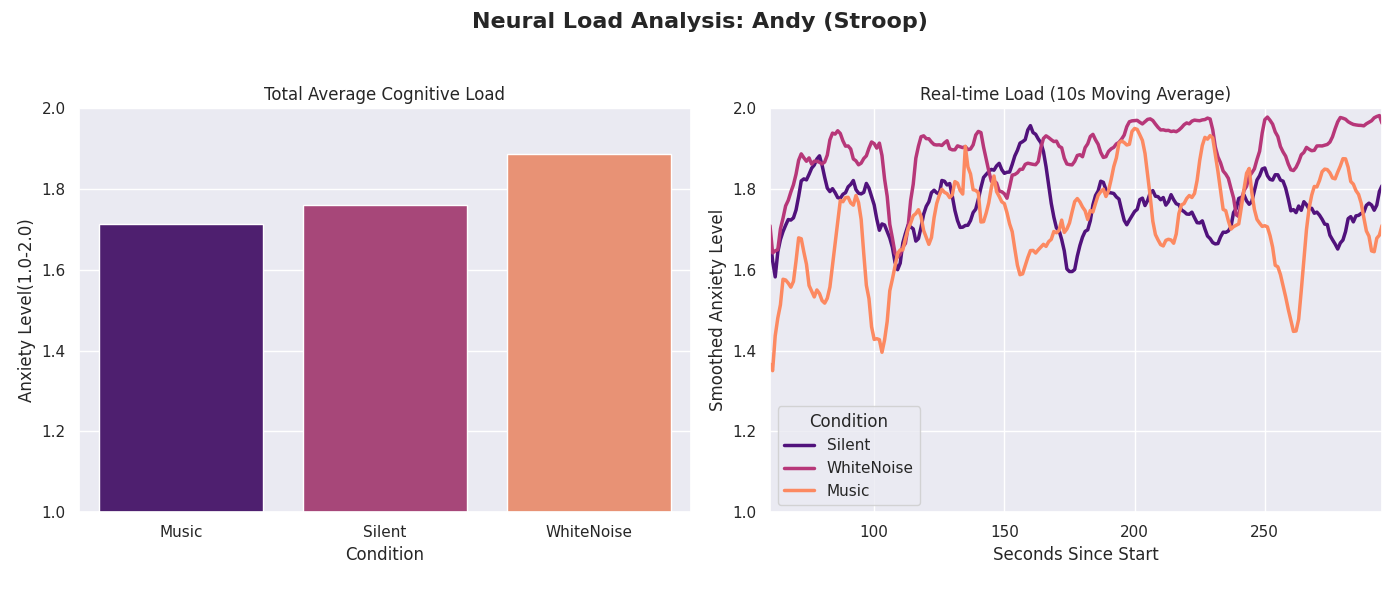
\includegraphics[width=\linewidth]{figures/neural_load_analysis.png}
%     \caption{Overall and Real-Time Anxiety Level~\cite{jtof-dev_EE-499_2026}.}
%     \label{fig:graph1}
% \end{figure}
%     \vfill
%
%     \begin{minipage}[c][0.48\textheight][c]{\linewidth}
%         \centering
%         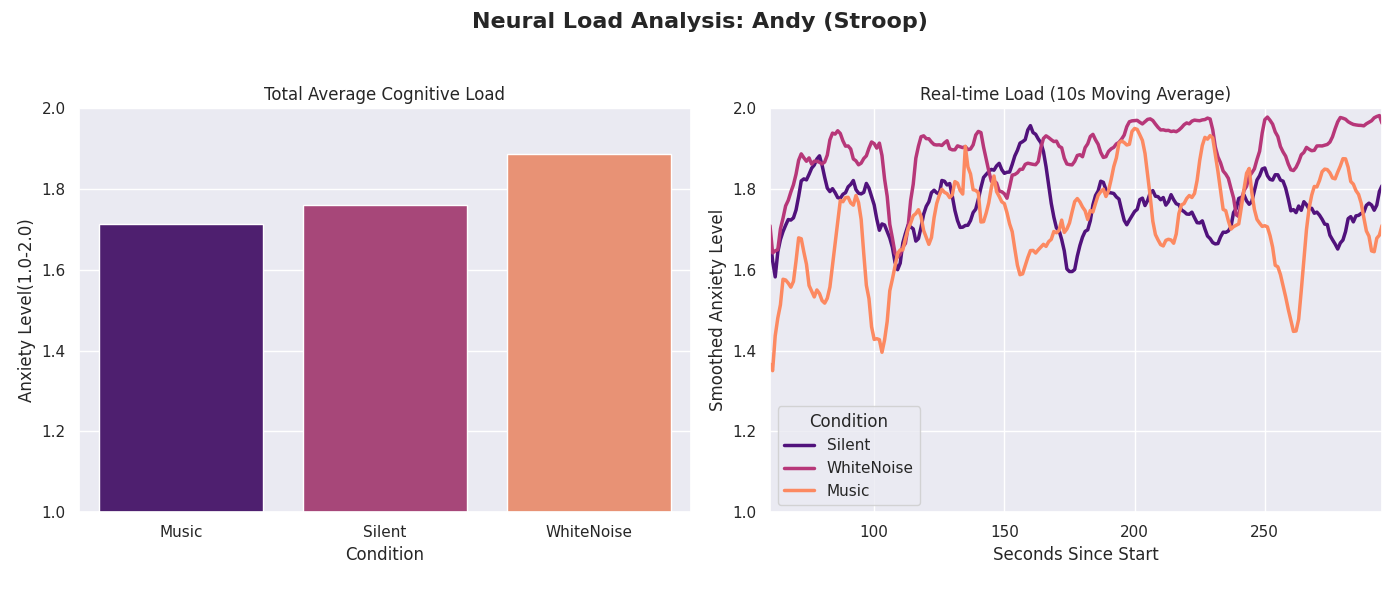
\includegraphics[width=\textwidth]{figures/neural_load_analysis.png}
%         \caption{Overall and Real-Time Anxiety Level~\cite{jtof-dev_EE-499_2026}.}
%         \label{fig:graph1}
%     \end{minipage}
% \end{figure*}

% ========
% ANALYSIS
% ========

\section{Analysis}

% focus on the most important concrete results - did sounds increase or decrease stress and performance, and give some graphs on that

Comparing the three auditory conditions shows an increase in total average correct answers and average keys pressed, with silence being the lowest and music the highest~\ref{tab:participant_andy_metrics_total}. However, the overall accuracy decreased during the music tests, with silence being the most accurate. It is possible that the increased anxiety level in the silent and white noise conditions cause enough second-guessing and slowdowns to prevent additional errors that music did not~\ref{fig:graph1}.

\begin{table}[htbp]
    \centering
    \caption{Aggregated Stroop test metrics for Andy. Data reflects total averages per run across different auditory conditions~\cite{jtof-dev_EE-499_2026}.}
    \label{tab:participant_andy_metrics_total}
    \resizebox{\linewidth}{!}{%
        \begin{tabular}{l c c c c c c}
            \toprule
            \textbf{Condition} & \textbf{Runs} & \textbf{Avg Keys} & \textbf{Avg Correct} & \textbf{Avg Errors} & \textbf{Keys/Sec} & \textbf{Accuracy (\%)} \\
            \midrule
            Silent     & 3 & 399.7 & 376.7 & 23.0 & 1.34 & 94.25 \\
            WhiteNoise & 2 & 432.5 & 403.0 & 29.5 & 1.45 & 93.18 \\
            Music      & 2 & 491.0 & 448.0 & 43.0 & 1.65 & 91.24 \\
            \bottomrule
        \end{tabular}%
    }
\end{table}

% ====================
% RESULTS & CONCLUSION
% ====================

\section{Results and Conclusion}

% compare my results to the papers I have cited in the paper and discuss whether or not those results are actually significant in any way
% then conclude

\bibliographystyle{IEEEtran}
\bibliography{references}

\end{document}
